Consider following unity gain feedback system, where there is a delay in the feedback path
\begin{center}
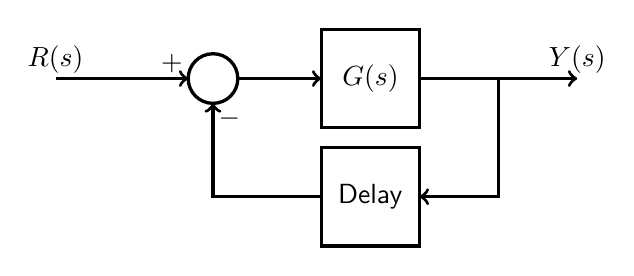
\begin{tikzpicture}[scale=1,inner sep=0pt,outer sep=0pt,very thick,
sysblock/.style={draw,rectangle,inner sep=2pt,minimum width=1.25cm,minimum height=1.25cm,inner sep=4pt, very thick}]
\draw (2,0) node[draw,circle] (sum1) {$\rule{0pt}{18pt}$};
\draw (4,0) node[sysblock] (G) {$G(s)$};
\draw (4,-1.5) node[sysblock] (delay) {\textsf{Delay}};
\draw[->] (0,0) node[above=2pt] {$R(s)$} -- (sum1.180) node[above left=2pt] {$+$};
\draw[->] (sum1.0)  -- (G.180);
\draw[->] (G.0) -- ++(2,0) node[above=2pt] {$Y(s)$};
\draw[->] (G.0) ++(1,0) |- (delay.0);
\draw[->] (delay.180) -| (sum1.-90) node[below right=2pt] {$-$};
\end{tikzpicture}
\end{center}
The following is the Bode plot of $G(s)$. 
\begin{center}
\includegraphics[width=5in]{\mainfolder/LectureNotes/\lecturefolder/HomeworkProblems/Problem07/bode2.pdf}
\end{center}
\begin{enumerate}[(a)]
\item Assume the delay is zero, and determine the phase and gain margin. Indicate on the Bode plot where this is measured.
\item Determine the maximum delay that can be tolerated before the system becomes unstable.
\end{enumerate}